%================================================================================
%       Safety Critical Systems Club - Data Safety Initiative Working Group
%================================================================================
%                       DDDD    SSSS  IIIII  W   W   GGGG
%                       D   D  S        I    W   W  G   
%                       D   D   SSS     I    W W W  G  GG
%                       D   D      S    I    WW WW  G   G
%                       DDDD   SSSS   IIIII  W   W   GGG
%================================================================================
%               Data Safety Guidance Document - LaTeX Source File
%================================================================================
%
% Description:
%   Radish - a tool to assist in applying the method.
%
%================================================================================
\chapter{The Data Safety Tool: RADISH\index{Radish|textbf} (Discursive)} \label{bkm:radish}
\dsiwgSectionQuote{Technology is nothing.
  What's important is that you have a faith in people, that they're basically good and smart, and if you give them tools, they'll do wonderful things with them.}{Steve Jobs}

\section{An introduction to the tool}
RADISH (The Risk Assessor for Data Integrity and Safety Hazards) is a software tool being developed by \href{https://mca-ltd.com/}{Mission Critical Applications Limited (mca-ltd.com)}, to assist a data safety practitioner developing a data safety case using the guidance, by:
\begin{itemize}
  \item recording the decisions that are made;
  \item automating parts of the data safety assessment process; and
  \item helping the practitioner to choose between the risk mitigations that are recommended by the guidance, given the nature of each risk.
\end{itemize}

For more information, and to access to the RADISH tool, visit \href{https://data-safety.tech/tooling}{data-safety.tech/tooling}.

As illustrated in \autoref{fig:radish}, the RADISH tool is a central repository of information about the data safety case for a project. RADISH guides data safety engineers to identify the data artefacts in the system, and the safety properties that are important for each artefact. It then calculates the highly recommended and recommended mitigation techniques following the guidance, allowing the engineer to chose those which should be in the system requirements those which should not, and record the justifications for those choices.

RADISH can generate reports showing the risks that have mitigations, and those where more work is needed, giving project management a view of the state of the data safety process. RADISH can also generate a report that can be included in a data safety case to support the system safety argument, and this can continue to evolve throughout the project lifecycle of development, deployment and maintenance.

\begin{figure}[htbp]
  \centering
  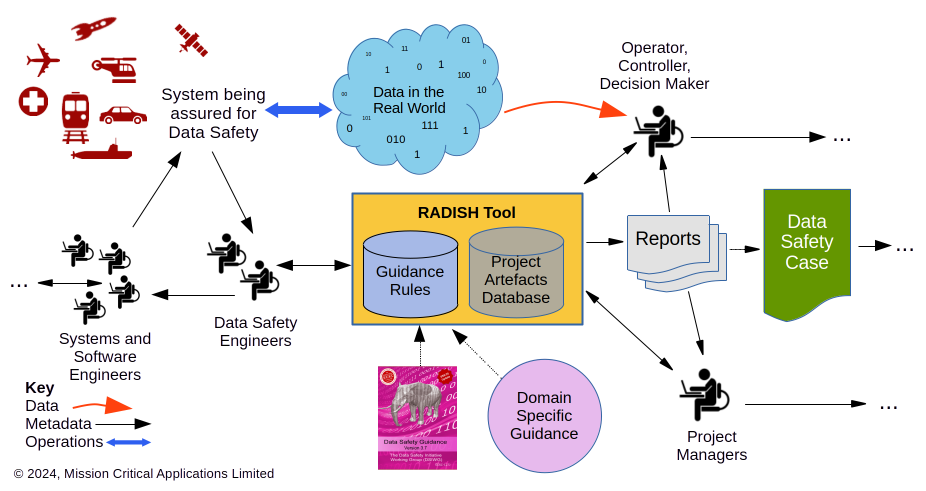
\includegraphics[angle=90,width=0.8\textwidth]{images/RADISH Tool in Project Environment - landscape.png}
  \caption{RADISH within the project environment\index{Radish context}}
  \label{fig:radish}
\end{figure}
\section{A caveat}
The tool described in this appendix is usable, but is not yet at production standard.
The developers are working towards a release in 2025, and are looking for programmes to use 
as test vehicles.
To have a programme considered as a possible test vehicle for the tool,
please contact the developers at
\href{mailto:radish@mca-ltd.com}{Mission Critical Applications Limited (radish@mca-ltd.com)}.
